
%% bare_conf.tex
%% V1.3
%% 2007/01/11
%% by Michael Shell
%% See:
%% http://www.michaelshell.org/
%% for current contact information.
%%
%% This is a skeleton file demonstrating the use of IEEEtran.cls
%% (requires IEEEtran.cls version 1.7 or later) with an IEEE conference paper.
%%
%% Support sites:
%% http://www.michaelshell.org/tex/ieeetran/
%% http://www.ctan.org/tex-archive/macros/latex/contrib/IEEEtran/
%% and
%% http://www.ieee.org/

%%*************************************************************************
%% Legal Notice:
%% This code is offered as-is without any warranty either expressed or
%% implied; without even the implied warranty of MERCHANTABILITY or
%% FITNESS FOR A PARTICULAR PURPOSE! 
%% User assumes all risk.
%% In no event shall IEEE or any contributor to this code be liable for
%% any damages or losses, including, but not limited to, incidental,
%% consequential, or any other damages, resulting from the use or misuse
%% of any information contained here.
%%
%% All comments are the opinions of their respective authors and are not
%% necessarily endorsed by the IEEE.
%%
%% This work is distributed under the LaTeX Project Public License (LPPL)
%% ( http://www.latex-project.org/ ) version 1.3, and may be freely used,
%% distributed and modified. A copy of the LPPL, version 1.3, is included
%% in the base LaTeX documentation of all distributions of LaTeX released
%% 2003/12/01 or later.
%% Retain all contribution notices and credits.
%% ** Modified files should be clearly indicated as such, including  **
%% ** renaming them and changing author support contact information. **
%%
%% File list of work: IEEEtran.cls, IEEEtran_HOWTO.pdf, bare_adv.tex,
%%                    bare_conf.tex, bare_jrnl.tex, bare_jrnl_compsoc.tex
%%*************************************************************************

% *** Authors should verify (and, if needed, correct) their LaTeX system  ***
% *** with the testflow diagnostic prior to trusting their LaTeX platform ***
% *** with production work. IEEE's font choices can trigger bugs that do  ***
% *** not appear when using other class files.                            ***
% The testflow support page is at:
% http://www.michaelshell.org/tex/testflow/



% Note that the a4paper option is mainly intended so that authors in
% countries using A4 can easily print to A4 and see how their papers will
% look in print - the typesetting of the document will not typically be
% affected with changes in paper size (but the bottom and side margins will).
% Use the testflow package mentioned above to verify correct handling of
% both paper sizes by the user's LaTeX system.
%
% Also note that the "draftcls" or "draftclsnofoot", not "draft", option
% should be used if it is desired that the figures are to be displayed in
% draft mode.
%
\documentclass[conference]{IEEEtran}
% Add the compsoc option for Computer Society conferences.
%
% If IEEEtran.cls has not been installed into the LaTeX system files,
% manually specify the path to it like:
% \documentclass[conference]{../sty/IEEEtran}





% Some very useful LaTeX packages include:
% (uncomment the ones you want to load)


% *** MISC UTILITY PACKAGES ***
%
%\usepackage{ifpdf}
% Heiko Oberdiek's ifpdf.sty is very useful if you need conditional
% compilation based on whether the output is pdf or dvi.
% usage:
% \ifpdf
%   % pdf code
% \else
%   % dvi code
% \fi
% The latest version of ifpdf.sty can be obtained from:
% http://www.ctan.org/tex-archive/macros/latex/contrib/oberdiek/
% Also, note that IEEEtran.cls V1.7 and later provides a builtin
% \ifCLASSINFOpdf conditional that works the same way.
% When switching from latex to pdflatex and vice-versa, the compiler may
% have to be run twice to clear warning/error messages.






% *** CITATION PACKAGES ***
%
%\usepackage{cite}
% cite.sty was written by Donald Arseneau
% V1.6 and later of IEEEtran pre-defines the format of the cite.sty package
% \cite{} output to follow that of IEEE. Loading the cite package will
% result in citation numbers being automatically sorted and properly
% "compressed/ranged". e.g., [1], [9], [2], [7], [5], [6] without using
% cite.sty will become [1], [2], [5]--[7], [9] using cite.sty. cite.sty's
% \cite will automatically add leading space, if needed. Use cite.sty's
% noadjust option (cite.sty V3.8 and later) if you want to turn this off.
% cite.sty is already installed on most LaTeX systems. Be sure and use
% version 4.0 (2003-05-27) and later if using hyperref.sty. cite.sty does
% not currently provide for hyperlinked citations.
% The latest version can be obtained at:
% http://www.ctan.org/tex-archive/macros/latex/contrib/cite/
% The documentation is contained in the cite.sty file itself.






% *** GRAPHICS RELATED PACKAGES ***
%
\ifCLASSINFOpdf
  \usepackage[pdftex]{graphicx}
  % declare the path(s) where your graphic files are
  \graphicspath{{./pix/}}
  % and their extensions so you won't have to specify these with
  % every instance of \includegraphics
  \DeclareGraphicsExtensions{.pdf,.jpeg,.png,.jpg}
\else
  % or other class option (dvipsone, dvipdf, if not using dvips). graphicx
  % will default to the driver specified in the system graphics.cfg if no
  % driver is specified.
  % \usepackage[dvips]{graphicx}
  % declare the path(s) where your graphic files are
  % \graphicspath{{../eps/}}
  % and their extensions so you won't have to specify these with
  % every instance of \includegraphics
  % \DeclareGraphicsExtensions{.eps}
\fi
% graphicx was written by David Carlisle and Sebastian Rahtz. It is
% required if you want graphics, photos, etc. graphicx.sty is already
% installed on most LaTeX systems. The latest version and documentation can
% be obtained at: 
% http://www.ctan.org/tex-archive/macros/latex/required/graphics/
% Another good source of documentation is "Using Imported Graphics in
% LaTeX2e" by Keith Reckdahl which can be found as epslatex.ps or
% epslatex.pdf at: http://www.ctan.org/tex-archive/info/
%
% latex, and pdflatex in dvi mode, support graphics in encapsulated
% postscript (.eps) format. pdflatex in pdf mode supports graphics
% in .pdf, .jpeg, .png and .mps (metapost) formats. Users should ensure
% that all non-photo figures use a vector format (.eps, .pdf, .mps) and
% not a bitmapped formats (.jpeg, .png). IEEE frowns on bitmapped formats
% which can result in "jaggedy"/blurry rendering of lines and letters as
% well as large increases in file sizes.
%
% You can find documentation about the pdfTeX application at:
% http://www.tug.org/applications/pdftex





% *** MATH PACKAGES ***
%
%\usepackage[cmex10]{amsmath}
% A popular package from the American Mathematical Society that provides
% many useful and powerful commands for dealing with mathematics. If using
% it, be sure to load this package with the cmex10 option to ensure that
% only type 1 fonts will utilized at all point sizes. Without this option,
% it is possible that some math symbols, particularly those within
% footnotes, will be rendered in bitmap form which will result in a
% document that can not be IEEE Xplore compliant!
%
% Also, note that the amsmath package sets \interdisplaylinepenalty to 10000
% thus preventing page breaks from occurring within multiline equations. Use:
%\interdisplaylinepenalty=2500
% after loading amsmath to restore such page breaks as IEEEtran.cls normally
% does. amsmath.sty is already installed on most LaTeX systems. The latest
% version and documentation can be obtained at:
% http://www.ctan.org/tex-archive/macros/latex/required/amslatex/math/





% *** SPECIALIZED LIST PACKAGES ***
%
%\usepackage{algorithmic}
% algorithmic.sty was written by Peter Williams and Rogerio Brito.
% This package provides an algorithmic environment fo describing algorithms.
% You can use the algorithmic environment in-text or within a figure
% environment to provide for a floating algorithm. Do NOT use the algorithm
% floating environment provided by algorithm.sty (by the same authors) or
% algorithm2e.sty (by Christophe Fiorio) as IEEE does not use dedicated
% algorithm float types and packages that provide these will not provide
% correct IEEE style captions. The latest version and documentation of
% algorithmic.sty can be obtained at:
% http://www.ctan.org/tex-archive/macros/latex/contrib/algorithms/
% There is also a support site at:
% http://algorithms.berlios.de/index.html
% Also of interest may be the (relatively newer and more customizable)
% algorithmicx.sty package by Szasz Janos:
% http://www.ctan.org/tex-archive/macros/latex/contrib/algorithmicx/




% *** ALIGNMENT PACKAGES ***
%
\usepackage{array}
% Frank Mittelbach's and David Carlisle's array.sty patches and improves
% the standard LaTeX2e array and tabular environments to provide better
% appearance and additional user controls. As the default LaTeX2e table
% generation code is lacking to the point of almost being broken with
% respect to the quality of the end results, all users are strongly
% advised to use an enhanced (at the very least that provided by array.sty)
% set of table tools. array.sty is already installed on most systems. The
% latest version and documentation can be obtained at:
% http://www.ctan.org/tex-archive/macros/latex/required/tools/


%\usepackage{mdwmath}
%\usepackage{mdwtab}
% Also highly recommended is Mark Wooding's extremely powerful MDW tools,
% especially mdwmath.sty and mdwtab.sty which are used to format equations
% and tables, respectively. The MDWtools set is already installed on most
% LaTeX systems. The lastest version and documentation is available at:
% http://www.ctan.org/tex-archive/macros/latex/contrib/mdwtools/


% IEEEtran contains the IEEEeqnarray family of commands that can be used to
% generate multiline equations as well as matrices, tables, etc., of high
% quality.


%\usepackage{eqparbox}
% Also of notable interest is Scott Pakin's eqparbox package for creating
% (automatically sized) equal width boxes - aka "natural width parboxes".
% Available at:
% http://www.ctan.org/tex-archive/macros/latex/contrib/eqparbox/





% *** SUBFIGURE PACKAGES ***
%\usepackage[tight,footnotesize]{subfigure}
% subfigure.sty was written by Steven Douglas Cochran. This package makes it
% easy to put subfigures in your figures. e.g., "Figure 1a and 1b". For IEEE
% work, it is a good idea to load it with the tight package option to reduce
% the amount of white space around the subfigures. subfigure.sty is already
% installed on most LaTeX systems. The latest version and documentation can
% be obtained at:
% http://www.ctan.org/tex-archive/obsolete/macros/latex/contrib/subfigure/
% subfigure.sty has been superceeded by subfig.sty.



%\usepackage[caption=false]{caption}
%\usepackage[font=footnotesize]{subfig}
% subfig.sty, also written by Steven Douglas Cochran, is the modern
% replacement for subfigure.sty. However, subfig.sty requires and
% automatically loads Axel Sommerfeldt's caption.sty which will override
% IEEEtran.cls handling of captions and this will result in nonIEEE style
% figure/table captions. To prevent this problem, be sure and preload
% caption.sty with its "caption=false" package option. This is will preserve
% IEEEtran.cls handing of captions. Version 1.3 (2005/06/28) and later 
% (recommended due to many improvements over 1.2) of subfig.sty supports
% the caption=false option directly:
\usepackage[caption=false,font=footnotesize]{subfig}
%
% The latest version and documentation can be obtained at:
% http://www.ctan.org/tex-archive/macros/latex/contrib/subfig/
% The latest version and documentation of caption.sty can be obtained at:
% http://www.ctan.org/tex-archive/macros/latex/contrib/caption/




% *** FLOAT PACKAGES ***
%
\usepackage{fixltx2e}
% fixltx2e, the successor to the earlier fix2col.sty, was written by
% Frank Mittelbach and David Carlisle. This package corrects a few problems
% in the LaTeX2e kernel, the most notable of which is that in current
% LaTeX2e releases, the ordering of single and double column floats is not
% guaranteed to be preserved. Thus, an unpatched LaTeX2e can allow a
% single column figure to be placed prior to an earlier double column
% figure. The latest version and documentation can be found at:
% http://www.ctan.org/tex-archive/macros/latex/base/



%\usepackage{stfloats}
% stfloats.sty was written by Sigitas Tolusis. This package gives LaTeX2e
% the ability to do double column floats at the bottom of the page as well
% as the top. (e.g., "\begin{figure*}[!b]" is not normally possible in
% LaTeX2e). It also provides a command:
%\fnbelowfloat
% to enable the placement of footnotes below bottom floats (the standard
% LaTeX2e kernel puts them above bottom floats). This is an invasive package
% which rewrites many portions of the LaTeX2e float routines. It may not work
% with other packages that modify the LaTeX2e float routines. The latest
% version and documentation can be obtained at:
% http://www.ctan.org/tex-archive/macros/latex/contrib/sttools/
% Documentation is contained in the stfloats.sty comments as well as in the
% presfull.pdf file. Do not use the stfloats baselinefloat ability as IEEE
% does not allow \baselineskip to stretch. Authors submitting work to the
% IEEE should note that IEEE rarely uses double column equations and
% that authors should try to avoid such use. Do not be tempted to use the
% cuted.sty or midfloat.sty packages (also by Sigitas Tolusis) as IEEE does
% not format its papers in such ways.





% *** PDF, URL AND HYPERLINK PACKAGES ***
%
%\usepackage{url}
% url.sty was written by Donald Arseneau. It provides better support for
% handling and breaking URLs. url.sty is already installed on most LaTeX
% systems. The latest version can be obtained at:
% http://www.ctan.org/tex-archive/macros/latex/contrib/misc/
% Read the url.sty source comments for usage information. Basically,
% \url{my_url_here}.

\usepackage[T1]{fontenc}
\usepackage[utf8]{inputenc}    % Allow portuguese accents (accute and circumflex)
%\usepackage{lmodern}




% *** Do not adjust lengths that control margins, column widths, etc. ***
% *** Do not use packages that alter fonts (such as pslatex).         ***
% There should be no need to do such things with IEEEtran.cls V1.6 and later.
% (Unless specifically asked to do so by the journal or conference you plan
% to submit to, of course. )


% correct bad hyphenation here
\hyphenation{op-tical net-works semi-conduc-tor}


\begin{document}
\title{FlatFish -- A compact subsea-resident\\ inspection AUV}

\author{
    \IEEEauthorblockN{Jan Albiez\IEEEauthorrefmark{1}\IEEEauthorrefmark{2}, 
    Sylvain Joyeux\IEEEauthorrefmark{1}, Christopher Gaudig\IEEEauthorrefmark{2}, 
    Jens Hilljegerdes\IEEEauthorrefmark{3}, Sven Kroffke\IEEEauthorrefmark{3}, 
    Christian Schoo\IEEEauthorrefmark{2}, \\
    Sascha Arnold\IEEEauthorrefmark{2}, Geovane Mimoso\IEEEauthorrefmark{1}, Pedro 
    Alcantara\IEEEauthorrefmark{1},   Rafael Saback\IEEEauthorrefmark{1}, 
    Joao Britto\IEEEauthorrefmark{1}, Diego Cesar\IEEEauthorrefmark{1}, \\
    Gustavo Neves\IEEEauthorrefmark{1}, Thomio Watanabe\IEEEauthorrefmark{1},
    Patrick Merz Paranhos\IEEEauthorrefmark{1}\IEEEauthorrefmark{2},
    Marco Reis\IEEEauthorrefmark{1},
    and Frank Kirchner\IEEEauthorrefmark{2}\IEEEauthorrefmark{3}\IEEEauthorrefmark{1}}
	\IEEEauthorblockA{\IEEEauthorrefmark{1}Brazilian Institute of Robotics, SENAI 
	CIMATEC, Salvador, Bahia, Brazil, Email: jan.albiez@fieb.org.br}
	\IEEEauthorblockA{\IEEEauthorrefmark{2}Robotics Innovation Center, DFKI GmbH, 
    Bremen, Germany}
	\IEEEauthorblockA{\IEEEauthorrefmark{3}Robotics Group, Universit\"at Bremen, 
	Bremen, Germany}
	}

% author names and affiliations
% use a multiple column layout for up to three different
% affiliations
%\author{\IEEEauthorblockN{Michael Shell}
%\IEEEauthorblockA{School of Electrical and\\Computer Engineering\\
%Georgia Institute of Technology\\
%Atlanta, Georgia 30332--0250\\
%Email: http://www.michaelshell.org/contact.html}
%\and
%\IEEEauthorblockN{Homer Simpson}
%\IEEEauthorblockA{Twentieth Century Fox\\
%Springfield, USA\\
%Email: homer@thesimpsons.com}
%\and
%\IEEEauthorblockN{James Kirk\\ and Montgomery Scott}
%\IEEEauthorblockA{Starfleet Academy\\
%San Francisco, California 96678-2391\\
%Telephone: (800) 555--1212\\
%Fax: (888) 555--1212}}

% conference papers do not typically use \thanks and this command
% is locked out in conference mode. If really needed, such as for
% the acknowledgment of grants, issue a \IEEEoverridecommandlockouts
% after \documentclass

% for over three affiliations, or if they all won't fit within the width
% of the page, use this alternative format:
% 
%\author{\IEEEauthorblockN{Michael Shell\IEEEauthorrefmark{1},
%Homer Simpson\IEEEauthorrefmark{2},
%James Kirk\IEEEauthorrefmark{3}, 
%Montgomery Scott\IEEEauthorrefmark{3} and
%Eldon Tyrell\IEEEauthorrefmark{4}}
%\IEEEauthorblockA{\IEEEauthorrefmark{1}School of Electrical and Computer Engineering\\
%Georgia Institute of Technology,
%Atlanta, Georgia 30332--0250\\ Email: see http://www.michaelshell.org/contact.html}
%\IEEEauthorblockA{\IEEEauthorrefmark{2}Twentieth Century Fox, Springfield, USA\\
%Email: homer@thesimpsons.com}
%\IEEEauthorblockA{\IEEEauthorrefmark{3}Starfleet Academy, San Francisco, California 
%96678-2391\\
%Telephone: (800) 555--1212, Fax: (888) 555--1212}
%\IEEEauthorblockA{\IEEEauthorrefmark{4}Tyrell Inc., 123 Replicant Street, Los Angeles, 
%California 90210--4321}}




% use for special paper notices
%\IEEEspecialpapernotice{(Invited Paper)}




% make the title area
\maketitle


\begin{abstract}
Currently the inspection of industrial underwater structures is performed by 
remotely operated vehicles or by divers. Since the number of underwater structures keeps growing, e.g. due to new oil and gas fields or offshore wind farms, the need for a 
constantly available method to inspect these structures arises. The FlatFish project is an initiative of BG Group Brazil and the Brazilian Institute of Robotics in Salvador and aims at developing a subsea-resident AUV which can inspect the infrastructure at an oil and gas site on demand. FlatFish is a compact AUV, designed to acquire a 
high-resolution, textured 3D model of an underwater structure within an oil and gas asset. 
FlatFish is very agile and can hover during inspection, it uses a novel kind of navigation 
system to safely reach its goal within the field and is designed to stay submerged for 
extended periods of time. Within this paper the system design of FlatFish is presented.
\end{abstract}

\IEEEpeerreviewmaketitle

\section{Introduction}

Underwater structures like oil and gas production systems or the foundations of buildings,
piers and off-shore wind facilities, have to be regularly inspected to evaluate the state
of the structure and to plan future interventions for repair and maintenance. These
inspections are currently performed by remotely operated vehicles (ROVs) or, if water depth and
availability allow it, by divers. Due to the fact that inspections of this kind require a
special support vessel, they are time-consuming, expensive, need to be planned a long time
in advance and rely on good weather conditions and seasonal constraints (e.g. not during
hurricane season or winter storms).

Especially when looking at subsea operations of the oil and gas industry, being able
to inspect the subsea part of an asset regularly and/or on demand plays a key role for
subsea asset integrity assurance (SIA) and integrity management. The key information gathered from inspections encompasses the general structural integrity and close visual data
(also known as close visual inspection, CVI). The former can be acquired by using sonars
from a greater distance. For the latter, a camera has to be brought close to the structure.
Being able to retrieve information on the current state of any subsea equipment within the
field whenever the need for an assessment arises, allows for much safer operations and a
reduction of the operational expenditures (OPEX) due to the ability to better plan asset
maintenance. While this already holds true for current offshore assets, it becomes crucial
for the planned deep sea assets or in future fields with more complex seafloor production
systems.

These kinds of inspections are logistically and financially not feasible with
ROVs since that would require the continuous presence of an ROV support vessel in the
field. There are very few installations with ROVs deployed from FPSOs, but the tether length 
limits the operational radius to an area around the FPSO. The
solution is the usage of autonomous underwater vehicles (AUVs) for in-field inspection.
\cite{gamechanger07} already predicted the increase of AUV capabilities and their use in
tasks beyond classic bathymetry.

AUV systems suitable for delivering the desired inspection data require enhanced capabilities.
The robot must be able to position its cameras and lights close to the inspection target
without damaging the structure. This requires an ROV-like maneuverability combined with a
control system maintaining safe operations. This hovering ability is one of the key
capabilities which is commonly used to distinguish bathymetry-class AUVs from 
inspection-class AUVs.

To guarantee that at any given time an inspection of the asset's subsea structures can be
performed, the AUV has to be readily available 24/7. Since deck space on platforms and FPSOs is
generally tight and to reduce the influence of the weather on operations, the solution is
to operate the AUV in a \textit{subsea-resident} mode. Within the AUV context, subsea-residency means that the robot has a dedicated docking station on the seafloor within the asset.
This docking station is connected to the topside facilities of the asset. While docked, the AUV can be charged, data can be downloaded from the AUV and mission
information can be uploaded to the AUV. When an inspection is required, the mission is
created on shore or topside and transmitted to the AUV. The AUV then leaves the docking
station, executes the mission and returns to the docking station to recharge the batteries
and transfer the inspection data.

Subsea-residency is not a new concept. The idea has already been appearing in research and
development for some time (e.g.~\cite{mcleod2011}). But until now the technology
for actually implementing a subsea-resident vehicle was not available. Subsea-residency originated 
from oceanographic research, where its intended use was to
expand the ranges of long-term environmental monitoring. Worldwide there are a few
projects ongoing which plan to use resident AUVs in the mid- to long-term, e.g.~\cite{german2012} or \cite{soltwedel2013}.

The requirements for a subsea-resident AUV and its support infrastructure are high.
All components have to be robust enough to be able to function even when being exposed 
to
the deep sea environment for extended periods. This includes corrosion,
bio-fouling, degradation of seals and the blockage of moving parts like thrusters and
locking mechanisms by sediments or other foreign objects. The AUV as well as the infrastructure have to be
designed in a way that on one hand addresses the aforementioned problems and on the other
hand allows for quick and cost efficient maintenance.

\subsection{Project FlatFish}

The FlatFish project is an initiative between BG Group Brazil and the Brazilian Institute
of Robotics (BIR) in Salvador and is funded through the Brazilian Government R\&D levy,
which requires 1\% of gross production revenue from large Brazilian oil and gas
fields to be invested in R\&D in Brazil.

FlatFish aims to develop a subsea-resident inspection AUV. The project is part
of a long-term research roadmap of BG Group Brazil in the area of robotics for oil and gas
production. The development of the AUV is divided into two phases: In the first phase the
development infrastructure in Brazil will be set up, the AUV will be designed and
integrated, and the first inspection tests will be conducted inshore off the coast of
Salvador, Brazil and in the maritime test tank at DFKI in Bremen, Germany. The second
phase will focus on extended offshore trials of the complete system, including the
docking station, within an asset of BG Group. Currently the project is at the end of the
first phase.

During a workshop between BG Group, BIR and DFKI at the beginning of the FlatFish project, the
scenario and the principal design parameters were defined. The scenario was defined as follows:

\begin{enumerate}
    \item The AUV resides within a docking station on the seafloor
    \item Topside sends a mission to inspect a specific structure within the asset,
        e.g.~a mainfold or an SSIV
    \item FlatFish leaves the docking station and navigates toward the specified structure using
        pipelines and other subsea structures as external references
    \item While in transit, FlatFish uses its onboard sensors to avoid obstacles and to record data of the asset's status (e.g.~pipelines or debris)
    \item At the inspection target, FlatFish uses an advanced camera system to perform a close
        visual inspection of the complete structure
    \item FlatFish returns to the docking station using the same navigation approach as before
    \item In the docking station the batteries are recharged, the data is downloaded to
        a topside server and a high-resolution video-linked 3D model is created as the inspection
        result.
\end{enumerate}

With this in mind, the basic requirements for the FlatFish AUV were set to the following:

\begin{itemize}
    \item Compact design with hovering capabilities
    \item Materials and mechanical design that allow for a long-term subsea deployment
    \item Extended sensor suite for highly detailed visual inspection
    \item Multi-modal navigation system tailored to use the asset's structure as landmarks
    \item Multiple tracking systems, e.g. pipeline tracking, cable tracking, structure
        tracking
    \item Online 3D reconstruction for adaptive inspection coverage and offline dense 3D
        reconstruction with referencing between video data and 3D model
\end{itemize}

This paper focuses on the FlatFish AUV. The developments within the project are shown in regard to the current state-of-the-art for inspection-class AUVs and the design of the AUV is
presented.

%%%%%%% here because of layout reasons
\begin{table}[!t]
% increase table row spacing, adjust to taste
\renewcommand{\arraystretch}{1.3}
% if using array.sty, it might be a good idea to tweak the value of
% \extrarowheight as needed to properly center the text within the cells
\caption{FlatFish -- Technical Data}
\label{tab:tech}
\centering
% Some packages, such as MDW tools, offer better commands for making tables
% than the plain LaTeX2e tabular which is used here.
\begin{tabular}{|l|l|}
\hline
Depth rating 	  & 300 m \\ \hline

Weight (in air)		& 275 kg \\ \hline

Size (LWH)			&	220 cm x 105 cm x 50 cm \\ \hline

Propulsion			& 6x 60N Enitech ring thrusters \\
 & (120N in each direction) \\ \hline

Battery	 			&  Lithium-Ion battery 5,8 kWh (11,6 kWh) @ 48V\\ \hline 

Communication & Rock7mobile RockBlock Iridium satellite modem (1,6 GHz) \\
(surface) 		& Digi XBee-Pro-868 (868 MHz)\\
 & ubiquiti PicoStation M2 HP WLAN-Modul (2,4 GHz) \\ \hline

Communication & Evologics S2CR 48/78 kHz \\
(submerged)	&	usable as USBL transponder \\ \hline

Communication & 10 GBit/s optical fibre \\
(tethered)			& 1 GBit/s Cat5e (max. 50m) \\ \hline


Light	& 4x Bowtech LED-K-3200 (3200 lumen each) \\ \hline

Laser Line & 2x Picotronic LD532-20-3(20x80)45-PL line laser \\
projector & 20mW each @ 532nm \\ \hline

Sonar	& BlueView MB1350-45 Multibeam Profiler (inspection sonar) \\
 & Tritech Gemini 720i Multibeam Imager (navigation sonar) \\
 & 2x Tritech Micron Sonar (obstacle avoidance) \\ \hline
  
Camera	& 4x Basler ace acA2040-gc25 \\
	& 2048x2048 at 25 frames/s, colour, GigabitEthernet \\\hline
	
Depthsensor & Paroscientific 8CDP700-I \\ \hline

INS/AHRS & KVH 1750 IMU \\ \hline

DVL &	Rowe SeaProfiler DualFrequency 300/1200 kHz \\ \hline
\end{tabular}
\end{table}

\begin{figure*}[!t]
	\begin{center}
		\centering
		\subfloat[bottom view]{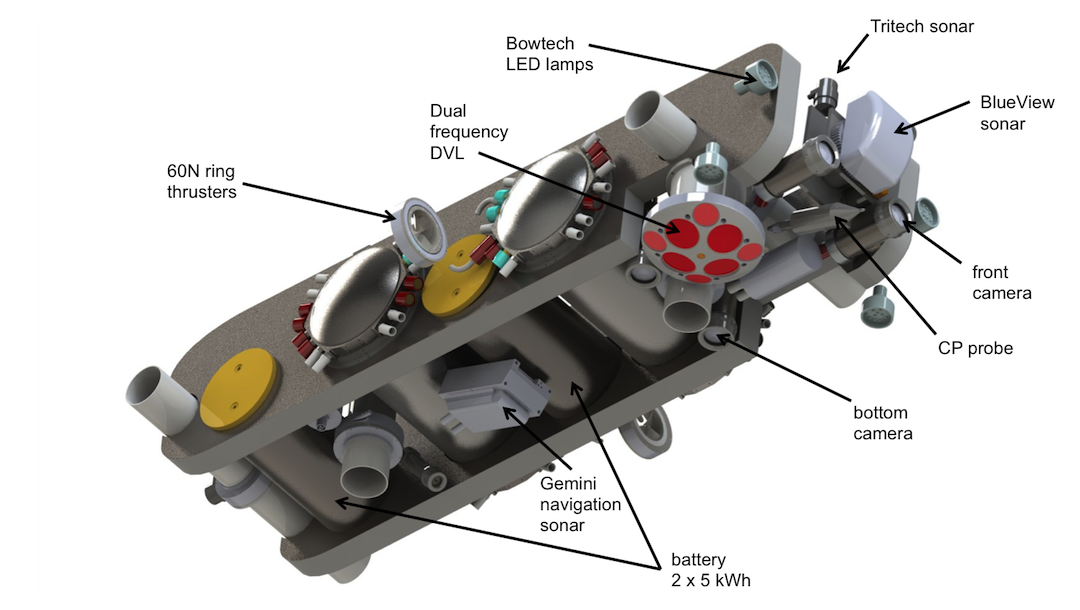
\includegraphics[width=0.5\textwidth]{flatfish_unten}}
		\hfil
		\subfloat[top view]{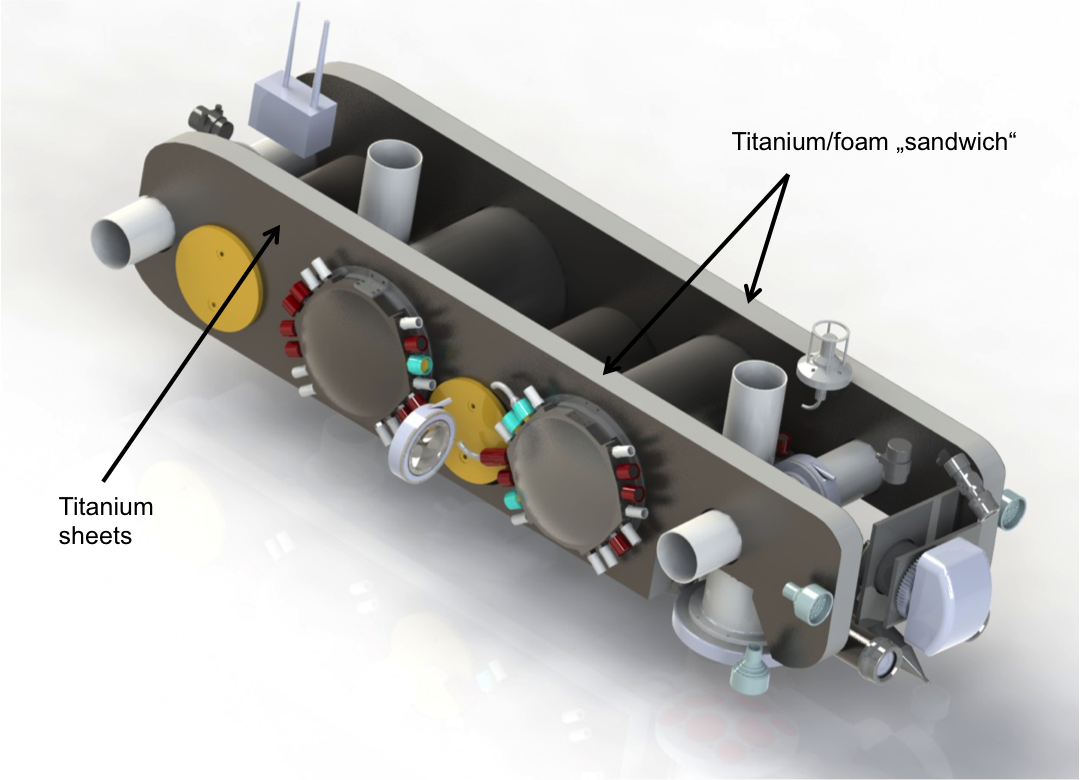
\includegraphics[width=0.5\textwidth]{flatfish_oben}}
		\caption{Placement of FlatFish's components (sensors, thrusters etc.)}
		\label{fig:sensor_placement}
	\end{center}
\end{figure*}
%%%%%%%

\section{Inspection-Class AUVs}

The primary task for autonomous underwater vehicles has always been data collection.
Initially, AUVs were designed to enhance the quality of sonar-based wide area surveys by
operating closer to the ground than a surface vessel and without the influence of waves. Up to this day
facilitating high-resolution bathymetric maps is still the primary application for AUVs.
Other wide area operations are the search for objects such as flight recorders (see
\cite{purcell2011}) or mine hunting (see \cite{Couillard2012}). AUVs designed to perform this
kind of tasks commonly use one propeller and control planes and therefore lack the
ability to \textit{hover}, meaning that they can't keep their position like ROVs. The
ability to hover is a key requirement to perform inspection tasks on complex structures.
Therefore this ability distinguishes inspection-class AUVs from mapping systems.

In recent years several AUV manufacturers developed prototypical modifications to their
mapping AUVs to perform inspection tasks, e.g.~the modified REMUS 500 presented in
\cite{packard2010}. All of these modifications have in common that hovering is relatively
expensive regarding energy consumption, so inspections which mainly rely on ROV-like motions are not
feasible with these systems.

SubSea 7's autonomous inspection vehicle (AIV) \cite{AIV} comes close to the requirements
defined for the FlatFish project. Nevertheless, the AIV mainly operates based on sonar, keeps longer distances to the inspection target and lacks the required high-resolution video system.

Lockheed Martin's Marlin \cite{Marlinmk1} is a large AUV primarily designed to carry a
bulky 3D imaging sonar. It has been used to perform optical surveys as well (see
\cite{mcleod2013}) but with mixed results. There have been some attempts to use the Saab
Seaeye Sabertooth \cite{johansson2010} as an inspection-class AUV, but it suffers from the
same size-related problems as the Marlin. 

There are several prototypes and single systems used in robotic or marine research.
Examples are the Italian TriMares \cite{cruz2011} used to evaluate dam inspection by AUVs,
the Spanish Girona 500 vehicle \cite{ribas2012} used in different European projects and
the Sentry AUV of the Woods Hole Oceanographic Institution in the USA, best known for its
work during the Deepwater Horizon accident \cite{Kinsey2011}. All these systems have in
common that they are unique solutions with special research interests.

A special case currently under development are so-called \textit{hybrid} ROVs, which
are hovering AUVs that are remotely controlled via a thin optical fiber during
the inspection/scientific part of their mission. The first known vehicle of this kind was
the deep-diving NEREUS \cite{bowen2009}. An example for a recent system is the HROV
\cite{meinecke2011} of the German MARUM.

The development in FlatFish is based on the work of the DFKI RIC on the design of
inspection AUVs. It mainly builds upon the operational experience with DAGON
\cite{hildebrandt2012} and on the mechatronic system of LENG \cite{hildebrandt2013}.

\section{Brazilian-German Development}

FlatFish is developed in a joint effort between the Robotics Innovation Center (RIC) of
DFKI in Bremen, Germany and the Brazilian Institute of Robotics (BIR) in Salvador,
Brazil. This cooperation creates the unique opportunity to combine the indoor testing
facilities and the experience with autonomous underwater robots in Bremen and the 
extensive testing opportunities and the emerging commercial and scientific market in Brazil.

The key elements of this cooperation within the project are the testing facilities which
complement each other, the joint development of hardware and software and the training of
researchers and other personnel.

The centerpiece of the maritime exploration
hall\footnote{http://robotik.dfki-bremen.de/en/research/research-facilities/maritime-exploration-hall.html}
at the facilities of DFKI RIC in Bremen is a 3.5 million liter saltwater test tank. This
tank allows for comprehensive tests of systems and control algorithms in a completely
controlled and safe environment. It is large enough for FlatFish to operate freely.

The coastal waters around Salvador have an average depth of approximately 30m and offer a
variety of different testing environments, close to offshore conditions with respect to
visibility and currents. The weather allows for nearly year-round testing with only a
short time in autumn (May to mid July) where high waves and thunderstorms can limit the
ability to test. 

Both locations will have their own FlatFish AUV. The first is being built in Bremen, the
second will be integrated in Salvador. Having two identical vehicles allows a seamless test,
evaluation and improvement of algorithms, hardware and operational procedures. E.g., a new algorithm for sensor processing can be tested in the clear water environment at the Bremen site and its principal functionality can be verified before it is tested in the ocean
environment in Salvador. The results of the tests in Salvador can then be analyzed at both
locations, any problems can be identified and the testing cycle can start again. With both
locations working in parallel this cycle can be very quick and efficient.

Working in a transcontinental cooperation forced the team to establish modern methods of
distributed development, change management, issue tracking, document management and
communication. The primary tool for coordinating the development work is
github\footnote{https://github.com/} which already brings all the tools needed to manage a
distributed team of software developers. In addition to github a build-server is used to
verify the current state of the software integration and
runrun.it\footnote{https://runrun.it/} is used to manage the tasks of the team members and
to coordinate the work between them. 

\section{The FlatFish AUV}

\subsection{Mechatronic Design}

The main goal of the FlatFish design was integrating all necessary sensors, the 
thrusters, the battery system and the electronics into a compact system. Early in the design 
phase the decision was made to use an open-frame design since it allows more freedom in 
placing components and sensors. Figure~\ref{fig:sensor_placement} shows the CAD model 
of the AUV without the cover to illustrate the placement of the components. The inspection 
sensors are described in section~\ref{sec:insp}, the navigation system is the topic of 
section~\ref{sec:nav}, all other components are described in more detail now.

\paragraph{\textbf{Frame, Support and Cover}} The frame features a titanium sheet
buoyancy foam composite and the launch and recovery hook support consists of welded titanium. 
This design allows for a very lightweight but still robust structure. The cover is made from 
fiberglass and its primary function is to reduce the potential points of entanglement while its 
secondary function is to reduce the hydrodynamic drag.

\paragraph{\textbf{Pressure Housings}} An analysis of the volume occupied by the electronics 
and the batteries showed that distributing the dry electronics into multiple smaller titanium 
pressure housings would reduce the size and weight of the housings. For 
reasons of modularity and weight distribution within the system, the batteries are placed in two 
pressure housings while the PCs, power electronics etc.~are 
distributed in two separate housings. The caps of the pressure housings are easy accessible from the 
side of the vehicle, thus facilitating maintenance.

\paragraph{\textbf{Propulsion System}} FlatFish is propelled by six hubless, pressure neutral 
ring thrusters. This type of thrusters is very robust with respect to extended underwater use 
and is able to withstand most kinds of debris without being blocked. The thrusters are 
configured in a rectangular configuration with two for each of the primary directions 
surge, heave and sway. This configuration is less agile than the ROV-type vectored thrust but 
much more efficient since full thrust is given in the desired direction of motion.

\paragraph{\textbf{Communication System}} FlatFish is equipped with a wide range of 
communication channels. All surface communication systems are gathered in a 
communications tower at the rear of the AUV which rises out of 
the water when FlatFish is surfaced. The comms tower is equipped with an Iridium satellite 
modem for worldwide communication, a GPS receiver, a 2.4GHz wireless LAN access point, 
an XBee Pro modem for redundancy and safety and a high-power LED beacon. For 
communication when submerged FlatFish is equipped with an acoustic modem. The comms tower 
can be configured to automatically transmit its GPS position via Iridium when it has satellite 
contact and it is equipped with its own backup battery.

It is possible to equip FlatFish with a short (100m) copper tether or a long fibre-optic cable 
turning it into a hybrid ROV. While this feature is not needed in the final application 
scenario it is a significant advantage during development.

\paragraph{\textbf{System Management}} All electrical components are connected to the 
power supply via electronic fuses, which are controlled by the system management board. 
The system management board is the part of FlatFish which controls the power to all other 
components in the system. It is the first component which powers up after a system start 
and the last component which switches off. The system management is directly connected 
to the XBee communication, acts as proxy for the underwater communication and controls 
the access to the propulsion system. The system management board itself is equipped with 
a watchdog and a brown-out circuit. Via the system management the AUV can activate, 
de-activate or reboot every component of FlatFish. The only exception being the battery-powered comms tower. 

This setup is the basis for a robust and fault-tolerant system, which is a necessity for 
long-term deployment. Every component of the AUV can be switched off in case of a 
major fault or be rebooted for fault recovery. Since the system management regulates 
access to the thrusters and can be contacted via every communication channel, the AUV 
can be forced to surface even when the main control software is malfunctioning. Also, FlatFish can be directly controlled at the surface via WiFi or XBee.

\begin{figure}[!t]
	\centering
	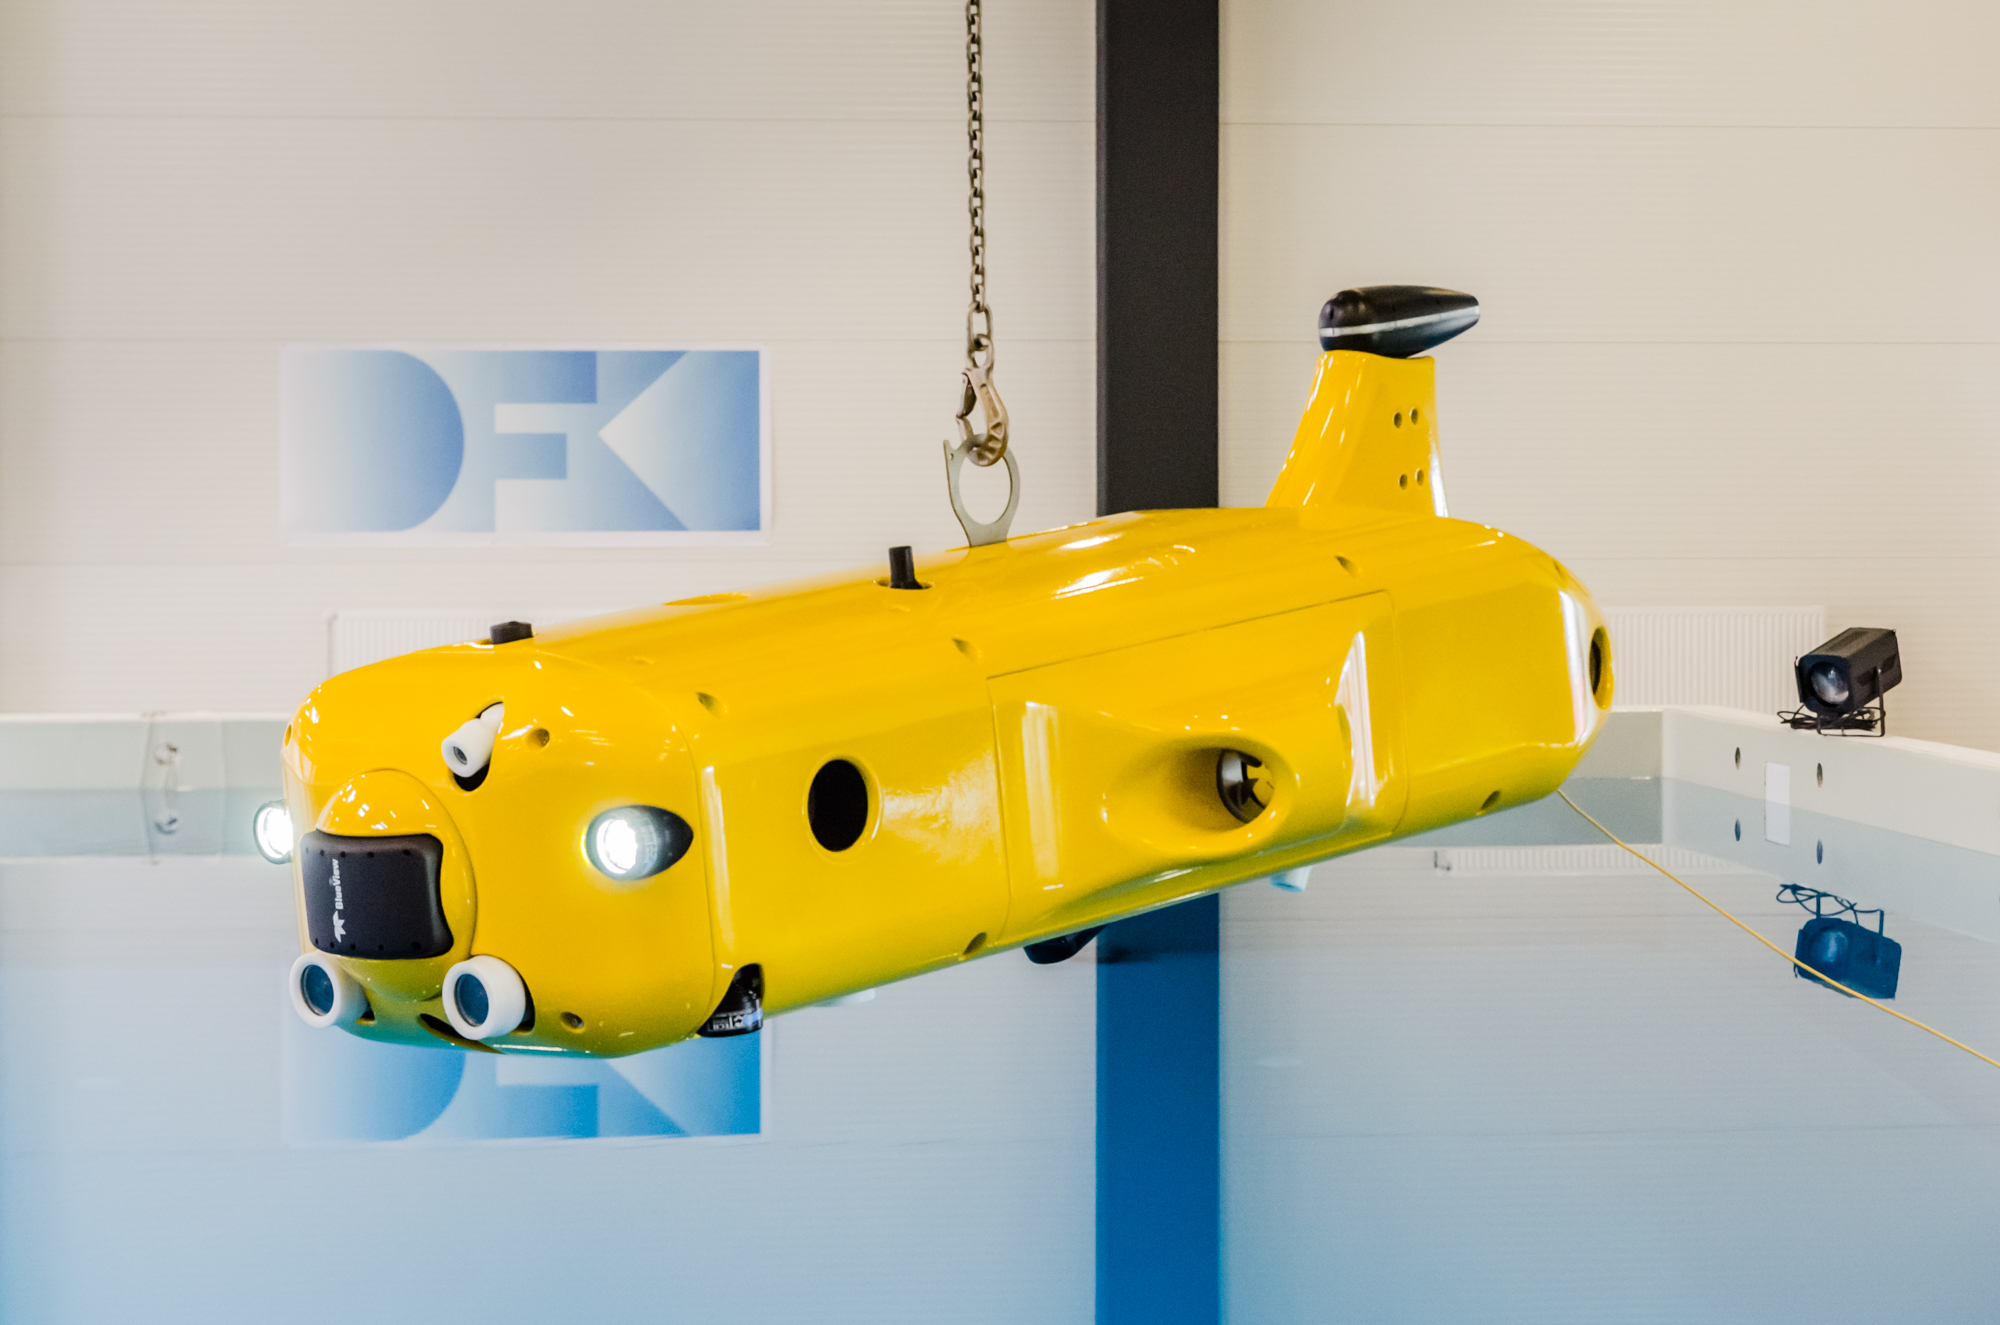
\includegraphics[width=0.9\columnwidth]{FlatFish-1.jpg}
	\caption{The completely integrated FlatFish at the DFKI RIC test facilities in Bremen, 
	Germany.}
	\label{fig:flatfish1}
\end{figure}

\paragraph{\textbf{Computer System}} FlatFish is equipped with two computers. 
One is the dedicated control PC which runs the low-level control, the navigation system 
and the mission management. The second PC is the payload system, and therefore is the 
host of the inspection software. The PCs are connected via Gigabit Ethernet which also acts 
as the main communication backbone.

Figure~\ref{fig:flatfish1} shows the fully integrated system at the DFKI facilities in Bremen.

\subsection{Software Architecture}

The vehicle's software architecture is based on the Robot Construction Kit
(Rock\footnote{http://rock-robotics.org/}), a component-based software integration
framework for robotics. The work done to use Rock on FlatFish is a continuation of
previous work, to which some of the authors contributed, on other AUVs~\cite{albiez2010}
and H-ROVs~\cite{meinecke2013}.

From the point of view of vehicle development, Rock provides the common set of tools
and services that is nowadays considered standard: visualization, logging (storing data), 
log replay (passing logged data to live components for testing) and state monitoring.
Where Rock differentiates itself is in its focus on robustness.

\begin{figure}[!t]
	\centering
	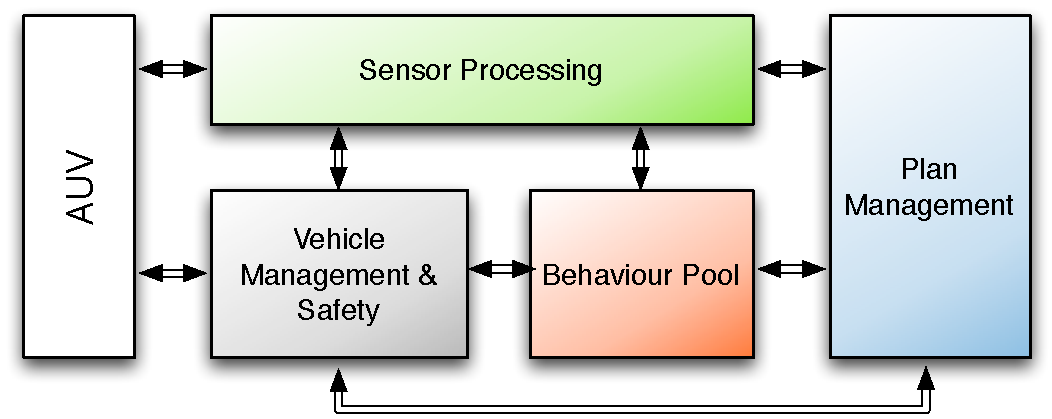
\includegraphics[width=0.9\columnwidth]{sw_arch_overview}
	\caption{High-level view of the FlatFish control architecture}
	\label{fig:sw_arch}
\end{figure}

Rock's architecture design supports the integration and \emph{coordination} of software
components that have a single purpose~\cite{Joyeux2013}, that is have a well-defined 
function that is as
stateless as possible. This contrasts with the common approach of ``fat components'',
whose behaviour very often depends on a lot of internal states, and is therefore hard to
assess externally. The components in the FlatFish architecture are meant to be designed
for a single purpose, which makes external diagnostic easier, and allows to make them
\emph{fail early}. The handling of these faults is then delegated to the system's
coordination layer, Syskit\cite{Joyeux2011}.

Syskit is a model-based approach designed to handle a component-based approach to 
data
processing in the robotic context~\ref{fig:sw_arch}. In addition to its diagnostic and fault 
recovery
aspects, it allows to design the different configurations of the system's component
networks, building a \emph{Behaviour Pool}, and then combine them in more complex 
systems
(correct-by-construction). At runtime, these various subsystems can then be switched on or
off when needed by the \emph{Plan Manager}, while leaving the details of which parts of
the software should be shut down or brought up to the model-based approach. This allows 
to
very easily provide hybrid ROV/AUV functionality, where any AUV functionality can be enabled or disabled by a ROV operator when needed, including fully autonomous mission
modes.

Given Syskit's complexity, the software architecture includes \emph{Vehicle Management
and Safety} functionality. This functionality, separated from the Syskit-based blocks, has
low autonomy. Its goal is to verify properties that are critical to the underwater asset's
integrity as well as the vehicle safety (the former having higher priority than the
latter). It can take over vehicle control to enter a safe mode when needed,
completely bypassing Syskit's own functions.

\subsection{Simulation}

In order to test the software integration and the mission and fault handling behaviours,
we have integrated the Gazebo realtime simulator~\footnote{http://gazebosim.org} into Rock.

Out of the box, Gazebo does not provide all the functionality required for FlatFish,
namely the following missing components:
\begin{itemize}
    \item water effect simulation for cameras, in particular the loss of color and the
        limited depth of view,
    \item physical effects of water (buoyancy, drag and added mass),
    \item simulation of different sonar types,
    \item the Rock integration
\end{itemize}

Our work consists firstly of a clean integration of Gazebo into the Rock framework, and
secondly its extension to support the simulation of an underwater environment. Technical
details about this integration can be found in~\cite{watanabe2015}.

\begin{figure}[!t]
	\centering
	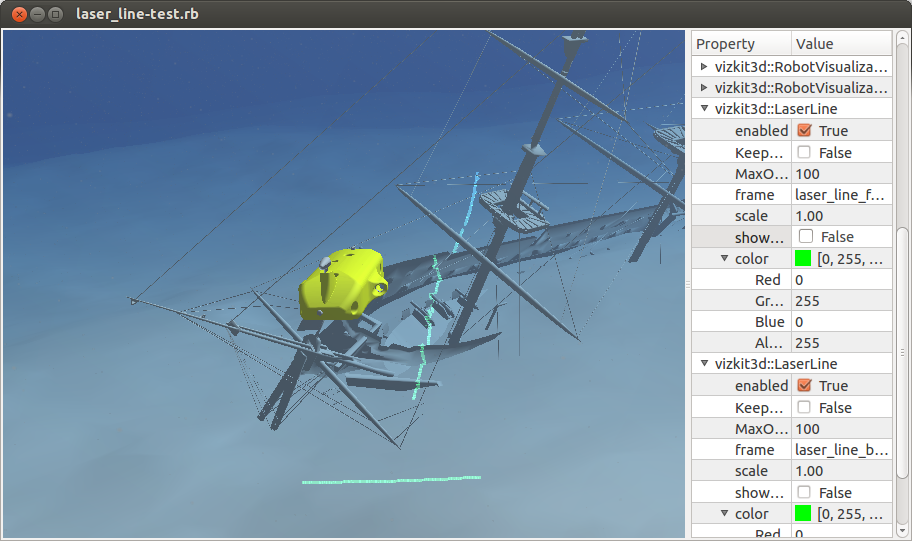
\includegraphics[width=0.9\columnwidth]{flatfish_simulation}
	\caption{Screenshot of the simulation with an active FlatFish using the laser line 
	projectors.}
	\label{fig:simulation}
\end{figure}


\subsection{Navigation System}
\label{sec:nav}

One of the largest problems for AUVs is a precise localization while en-route. Contrary to 
ROVs, an AUV normally has no base vessel which can localize it acoustically. An AUV solely 
has to rely on its INS and the DVL used with dead-reckoning to compute the current 
position and therefore accumulates an error over time. This error grows larger the 
more the AUV turns, a typical motion when performing an inspection. During some AUV missions 
a large baseline (LBL) transponder net is deployed to correct for errors 
(e.g.~\cite{purcell2011}), but setting up a LBL network is a major logistical effort.

The navigation system of FlatFish makes use of the installations and infrastructure within an 
offshore asset to guarantee safely reaching an inspection target, even if this target is 
located a long distance away from the docking station. Since every part of the asset is in some way connected to the platform or the FPSO, FlatFish uses these 
connections, normally pipelines or umbilicals, as navigation aids. Instead of an absolute 
global localization, FlatFish uses pipelines and umbilicals like roads connecting the individual 
parts of the asset. FlatFish metaphorically carries a map of the asset and uses it for navigation. This layout-aided navigation uses several modalities which are 
fused whenever they are applicable (see also figure \ref{fig:nav_overview}):
\paragraph*{\textbf{INS/DVL}} The fusion of the INS, the DVL and the vehicle's motion 
model into  a dead-reckoning system by using an Extended Kalman Filter (EKF)
\paragraph*{\textbf{USBL}} Within a 1km range from the docking station, the USBL/modem is 
used to help FlatFish find its dock. Current plans only have the docking 
station equipped with an USBL, but it is also possible to equip other parts of the asset (like 
manifolds) with a USBL repeater to further aid navigation.
\paragraph*{\textbf{Pipelines \& Umbilicals}} FlatFish possesses an advanced 
opto-acoustic pipeline and cable tracker. Using this tracking system, FlatFish can \textit{lock} onto the pipeline connecting its current inspection target with the rest 
of the asset and safely find it, even if the target is several kilometers away from the docking 
station. A further benefit of this tracking is, that a general visual inspection of the pipelines 
within the asset is done automatically.
\paragraph*{\textbf{Acoustic Feature Detection}} It is planned to use the forward-looking 
imaging sonar (Tritech Gemini 720i) to support the transition between the junction at the end of the 
pipelines/umbilicals and the current target of the navigation.
\paragraph*{\textbf{3D reconstruction/inspection}} The main part of the inspection data 
processing is done offline (see section \ref{sec:insp}), but the coverage check is done by an 
online algorithm. This part of the inspection system is used to localize the AUV with respect 
to the inspection target. This is of special importance since it is expected that the DVL 
will produce errors due to the close proximity to the structure, thus leaving the 
dead-reckoning in a critical state.

\begin{figure}[!t]
\begin{center}
	\subfloat[During transitions the INS/DVL-based localization is supported by tracking of 
	asset strucutres like flowlines 
	]{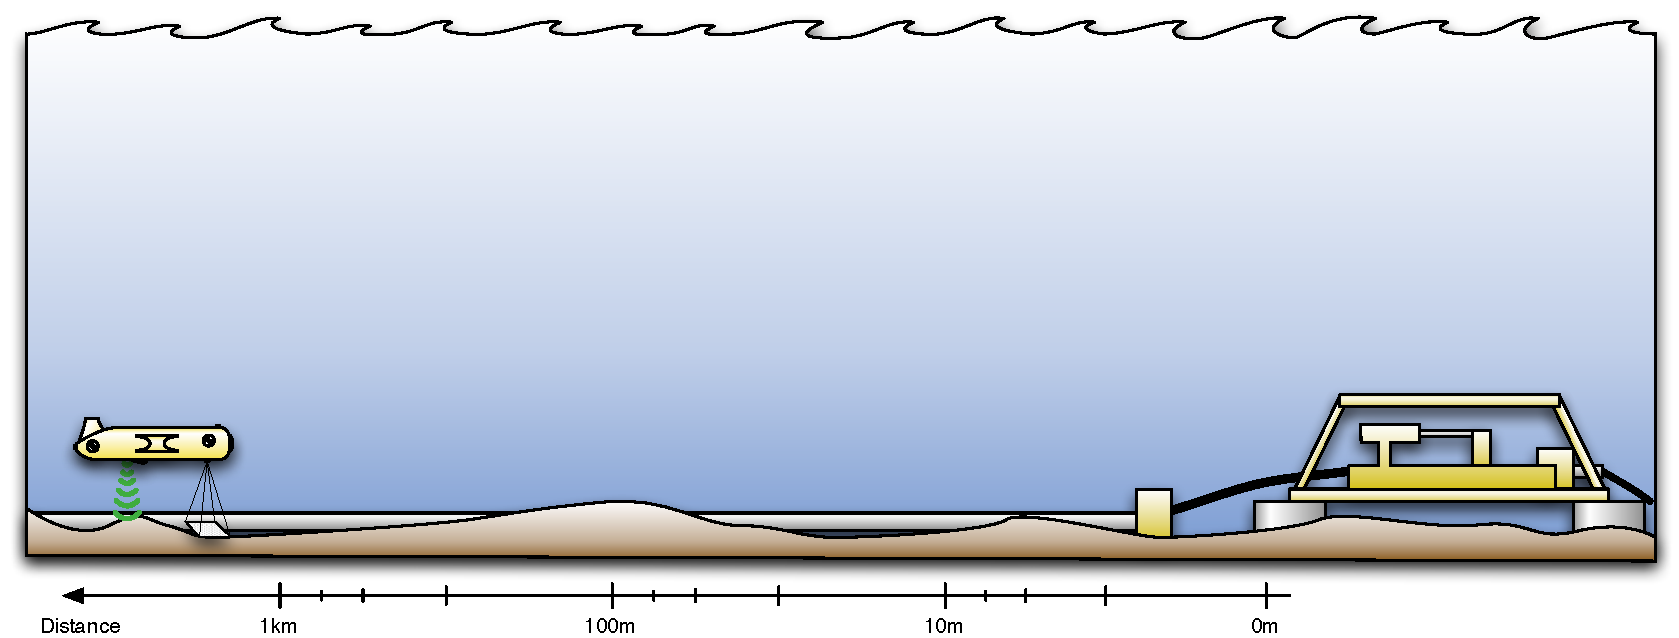
\includegraphics[width=\columnwidth]{FF-NavigationOverview-1}}\\
	\subfloat[Closer (less than 100 m) to major asset structures the forward-looking imaging 
	sonar and the obstacle avoidance sonar are used to localize the 
	structure]{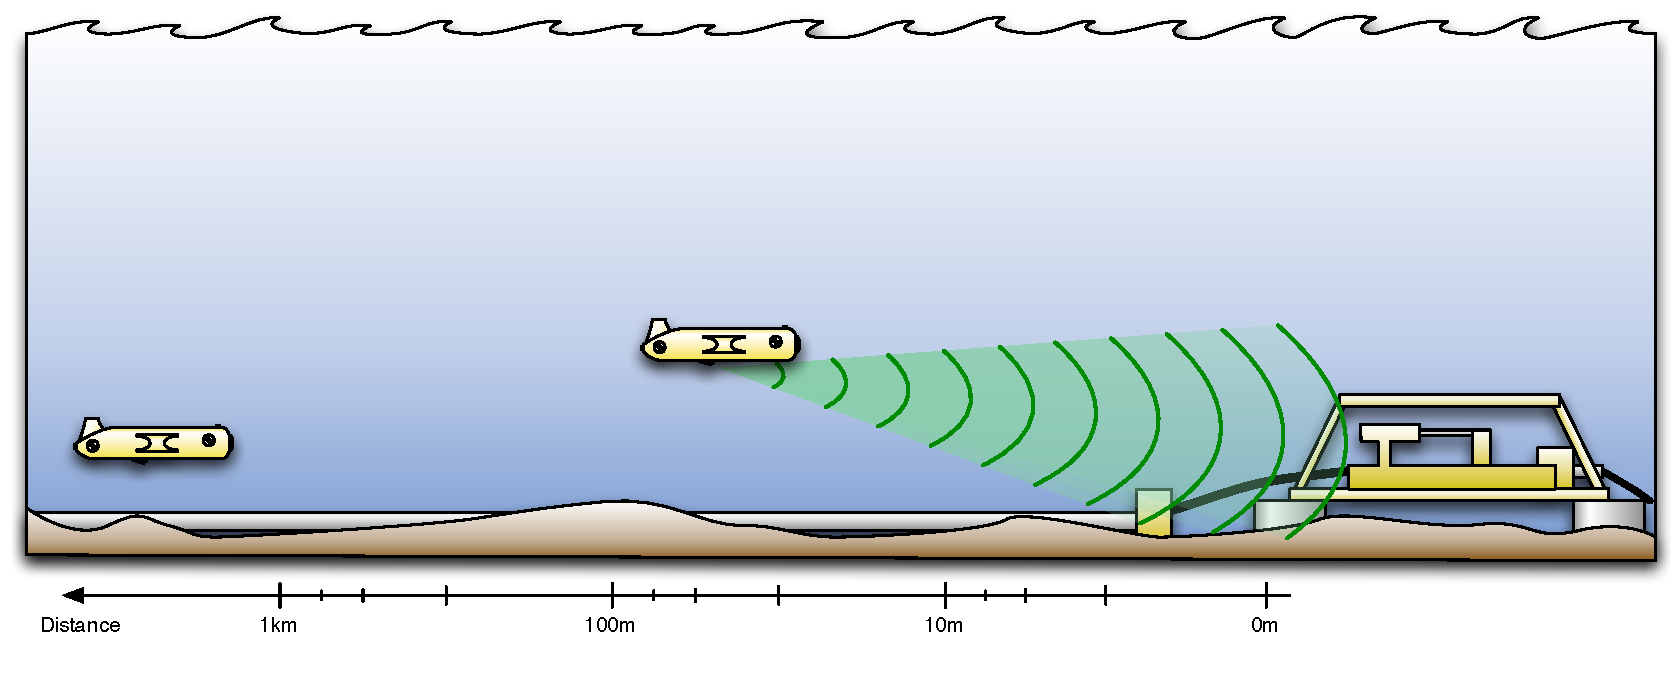
\includegraphics[width=\columnwidth]{FF-NavigationOverview-2}}\\
	\subfloat[During inspection the 3D reconstruction data (visual and sonar) is used to track 
	the AUV's relative position with respect to the structure 
	]{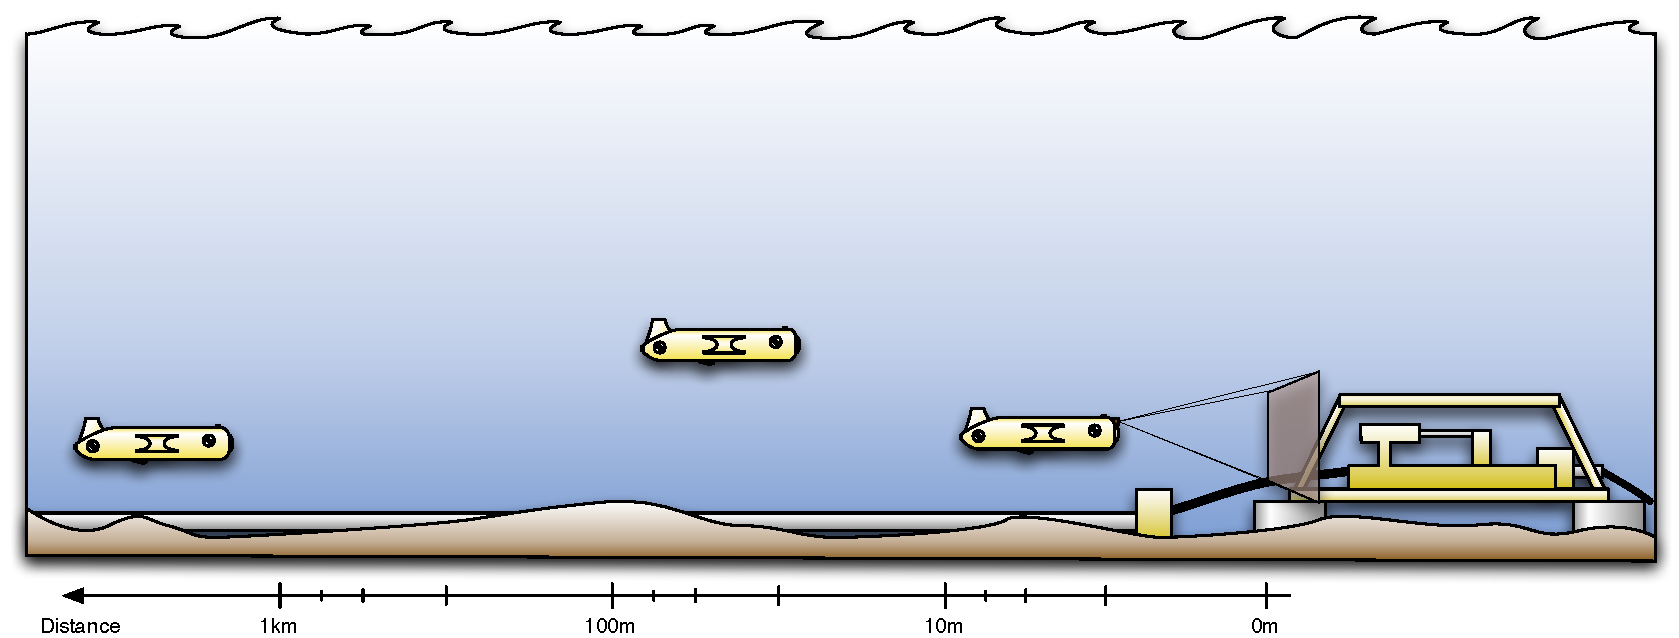
\includegraphics[width=\columnwidth]{FF-NavigationOverview-3}}\\
\caption{Overview of the three major navigation modalities for the layout-aided 
navigation of FlatFish }
\label{fig:nav_overview}
\end{center}
\end{figure}

The fusion of all these modalities into the final localization solution will be done by an EKF.

\subsection{Inspection System}
\label{sec:insp}

The inspection system is the key element of FlatFish. To fulfill the requirements 
regarding inspection data, a multi-modal approach was chosen. The idea behind this is 
to decrease the influence of the environmental conditions, mainly visibility, on the gathering 
of inspection data as much as possible.

The inspection sensor system consists of three sensor modalities, two optical and one 
acoustical:
\paragraph*{\textbf{Profiling Multi-Beam Sonar}} To allow a general inspection from greater 
distances or in very high turbidities (bad visibility), FlatFish is equipped with a high-resolution 
multi-beam profiling sonar (Blueview MB-1350). This sensor is mounted at the front of the AUV 
and can be turned by an electric rotator to change the orientation of the sonar fan between 
horizontal and vertical. By tracking the vehicle motion, the profiling sonar is used to generate 
a 3D model of the target structure in bad visibility and will be used as an 
additional modality for the visual inspection.

\paragraph*{\textbf{Stereo Camera Systems}} FlatFish is equipped with two stereo camera systems. 
One forward-looking system and one downward-looking system 
 also mounted in the front half of the AUV. Both systems use the same 2k Ethernet cameras 
(see table~\ref{tab:tech}) which are directly connected to the inspection PC. The 
camera systems are supplemented by a set of dimmable lamps each. The system is expected 
to work in conditions where the visibility range exceeds 2m. For higher turbidities the data acquired does not provide the 
quality required for the inspection. The stereo cameras are used in conjunction with a 
structure-for-motion algorithm to generate a high-resolution, textured 3D model of the 
structure to be inspected.

\paragraph*{\textbf{Laser Line Projection}} FlatFish features two green laser line projectors (20mW@532nm) which can be switched on by software and project a laser line 
onto the image of each of the stereo cameras (see figure~\ref{fig:flatfishlaser}). With the help 
of an automatic extraction system 
(see \cite{duda2013}) and by tracking the motion of AUV, the laser line is used to generate a 
3D model of the inspection target (e.g.~like in \cite{mcleod2013}). The advantage of the 
laser line projector is, that it works even in high turbidities (see \cite{albiez2015}). But even under
good visibility conditions it can support the stereo system by providing exact distances to a target.

The inspection itself is pre-planned by using either the CAD model of the structure or a 
model from a previous run. While inspecting, an online model is generated which is used for 
navigation and for verifying the coverage of the structure. After the return of the AUV to the 
docking station and the transfer of the data to topside, this model is used as the basis for 
generating the high-resolution inspection model. This inspection model is linked to all the raw 
data used to generate it (e.g.~videos) and allows the operators of the asset to do a structure-based browsing of the inspection results.

\begin{figure}[!t]
	\centering
	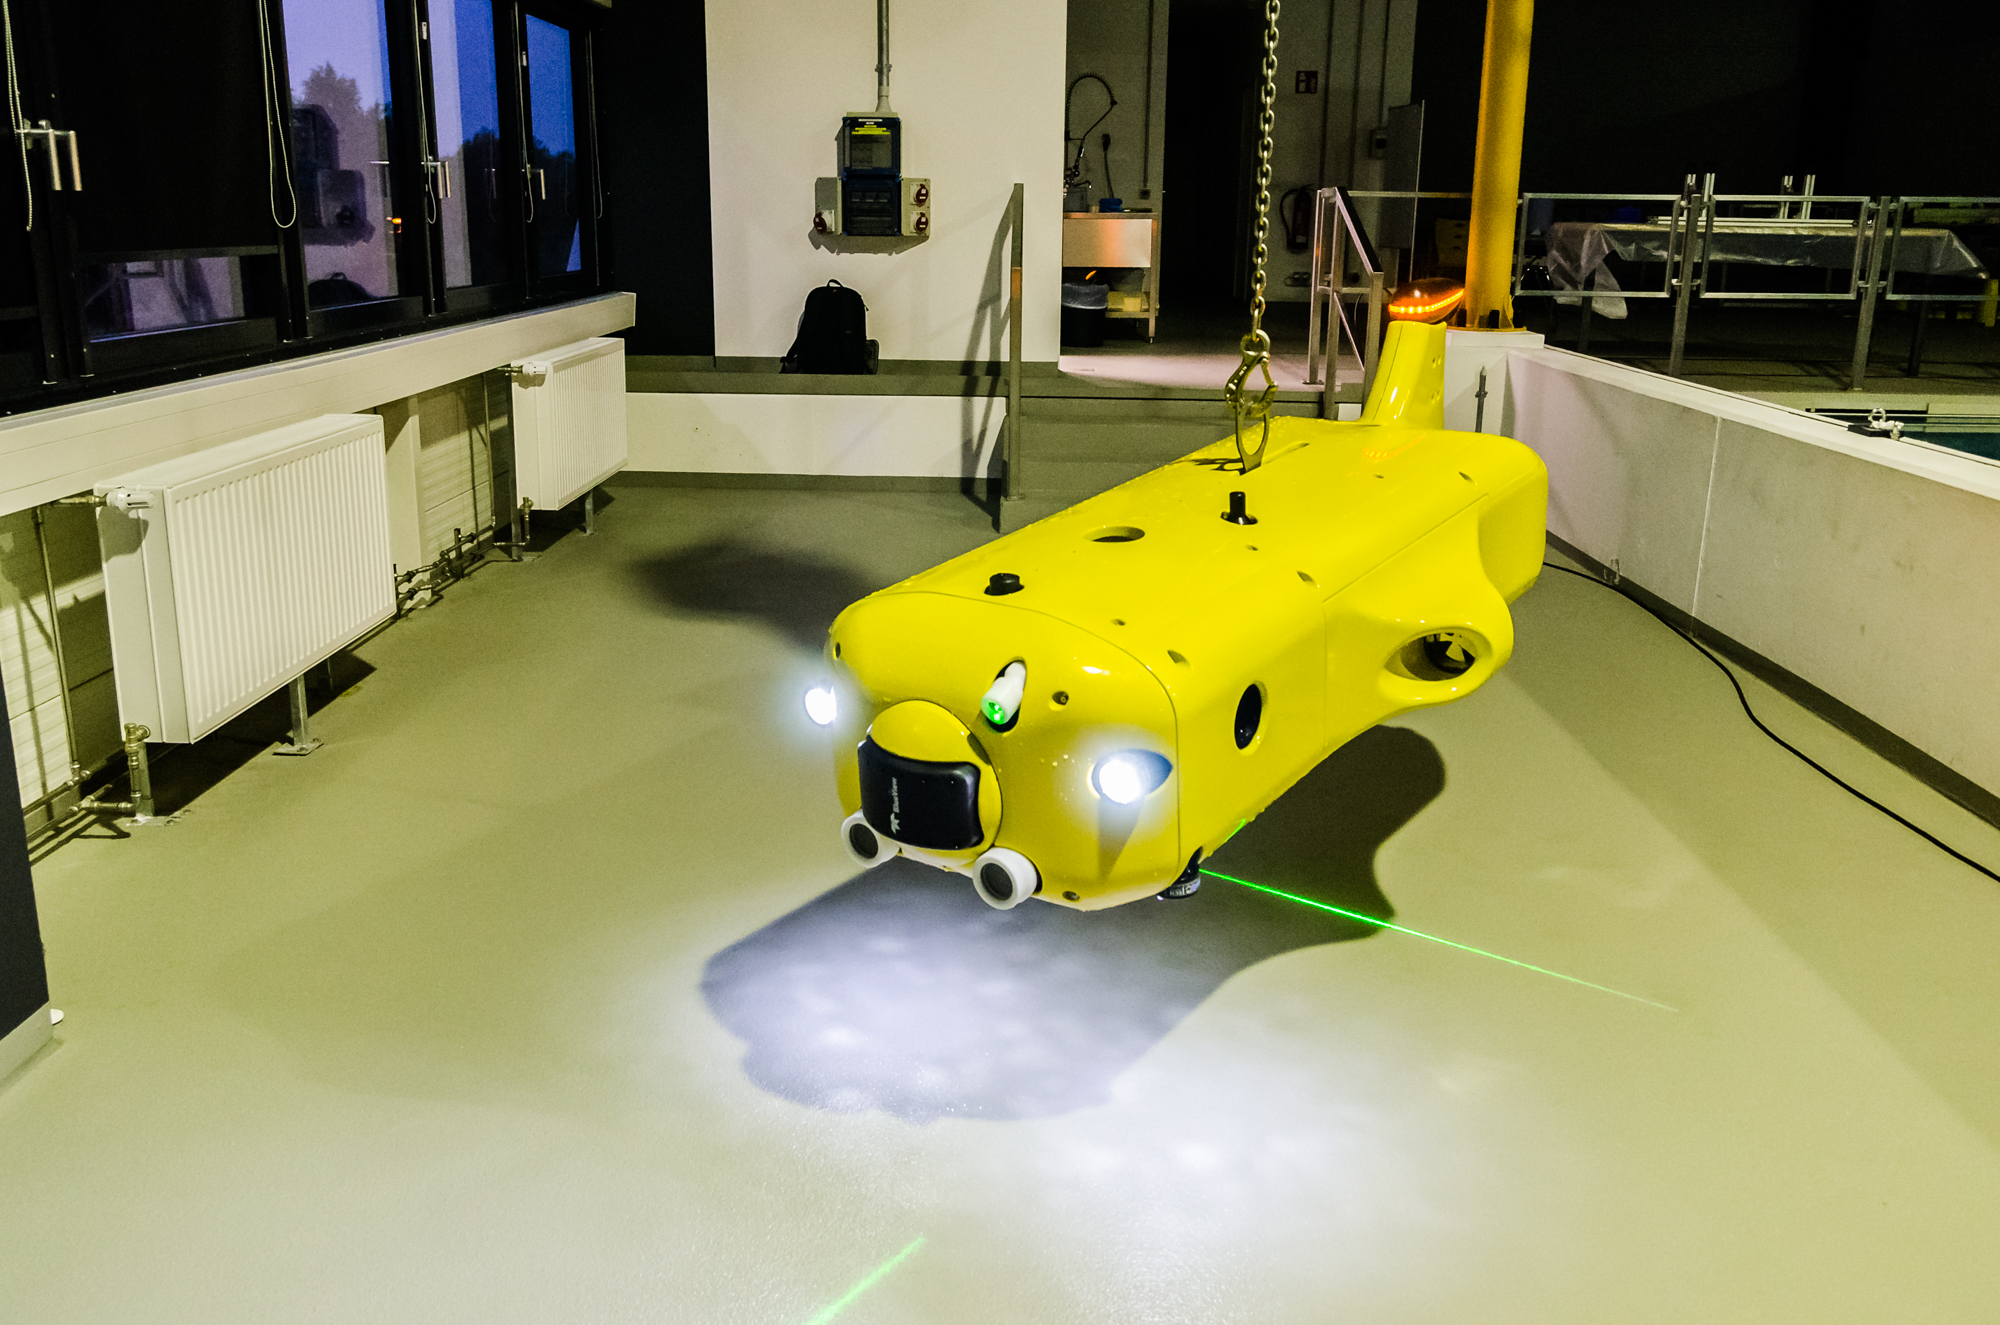
\includegraphics[width=0.9\columnwidth]{FlatFish-3.jpg}
	\caption{FlatFish attached to the crane at DFKI in Bremen. The green 
	lines of the laser projectors under and in front of the AUV can be seen. On the front of the AUV the 
	BlueView inspection sonar, the lights and the forward-looking stereo camera system is 
	visible.}
	\label{fig:flatfishlaser}
\end{figure}


\section{Integration Tests}

In June 2015 the integration of the first vehicle was finished in Bremen, Germany and a
series of specification compliance tests was performed by BIR scientists together with the 
staff at DFKI. The goal of these tests was to check whether the fully integrated AUV 
complies with the specifications regarding the mechatronic system and the basic motion 
capabilities. 

The tests were performed in the large saltwater tank of the maritime exploration hall in Bremen.
A mock-up of a pipeline was installed as a visual target for the vehicle and the
experiments were documented using a Mini-ROV (see figure \ref{fig:flatfish2}). 

The tests consisted of a series of tracks which FlatFish had to follow using the
INS/DVL-based dead-reckoning pose estimator and the waypoint-following behaviour. The
pipeline mock-up was the target for testing the downward-looking camera system and was 
used as a the test object for the pipeline detector. The FlatFish AUV was able to successfully
fulfill all parts of the test. The waypoint navigation autonomously followed a set of
waypoints in the tank over a time period of 30 minutes. All sensors of FlatFish
worked correctly and the pipeline detector was able to detect the pipeline whenever
FlatFish crossed it. 

\section{Conclusion}

The FlatFish AUV is the first step towards an integrated subsea-resident inspection system for
offshore oil and gas. The design and testing philosophy using a multinational team was 
presented, the mechatronic design introduced and the navigation and inspection 
systems outlined. 

The specification compliance tests done at the DFKI RIC in Bremen,
Germany showed that the mechatronic design of FlatFish is in accordance to the 
specification. The next step in the project consists of extensive tests inshore off the coast of 
Salvador with the Brazilian FlatFish. As inspection target one of the various shipwrecks in 
the Bahian waters will be chosen, since the process to qualify FlatFish to work in an offshore 
asset is still ongoing. 

In parallel, the design and integration of the docking station prototype will be done. The 
tests of the docking process will primarily be performed in the clear saltwater tank in Bremen.

Future work on FlatFish will focus on qualification of FlatFIsh for offshore assets, enhancing 
the inspection capabilities, performing field trials in an offshore oil and gas asset and enhancing 
the navigation system by incorporating new methods like magnetic tracking 
\cite{christensen2015} and increasing the level of autonomy. 

\begin{figure}[!t]
	\centering
	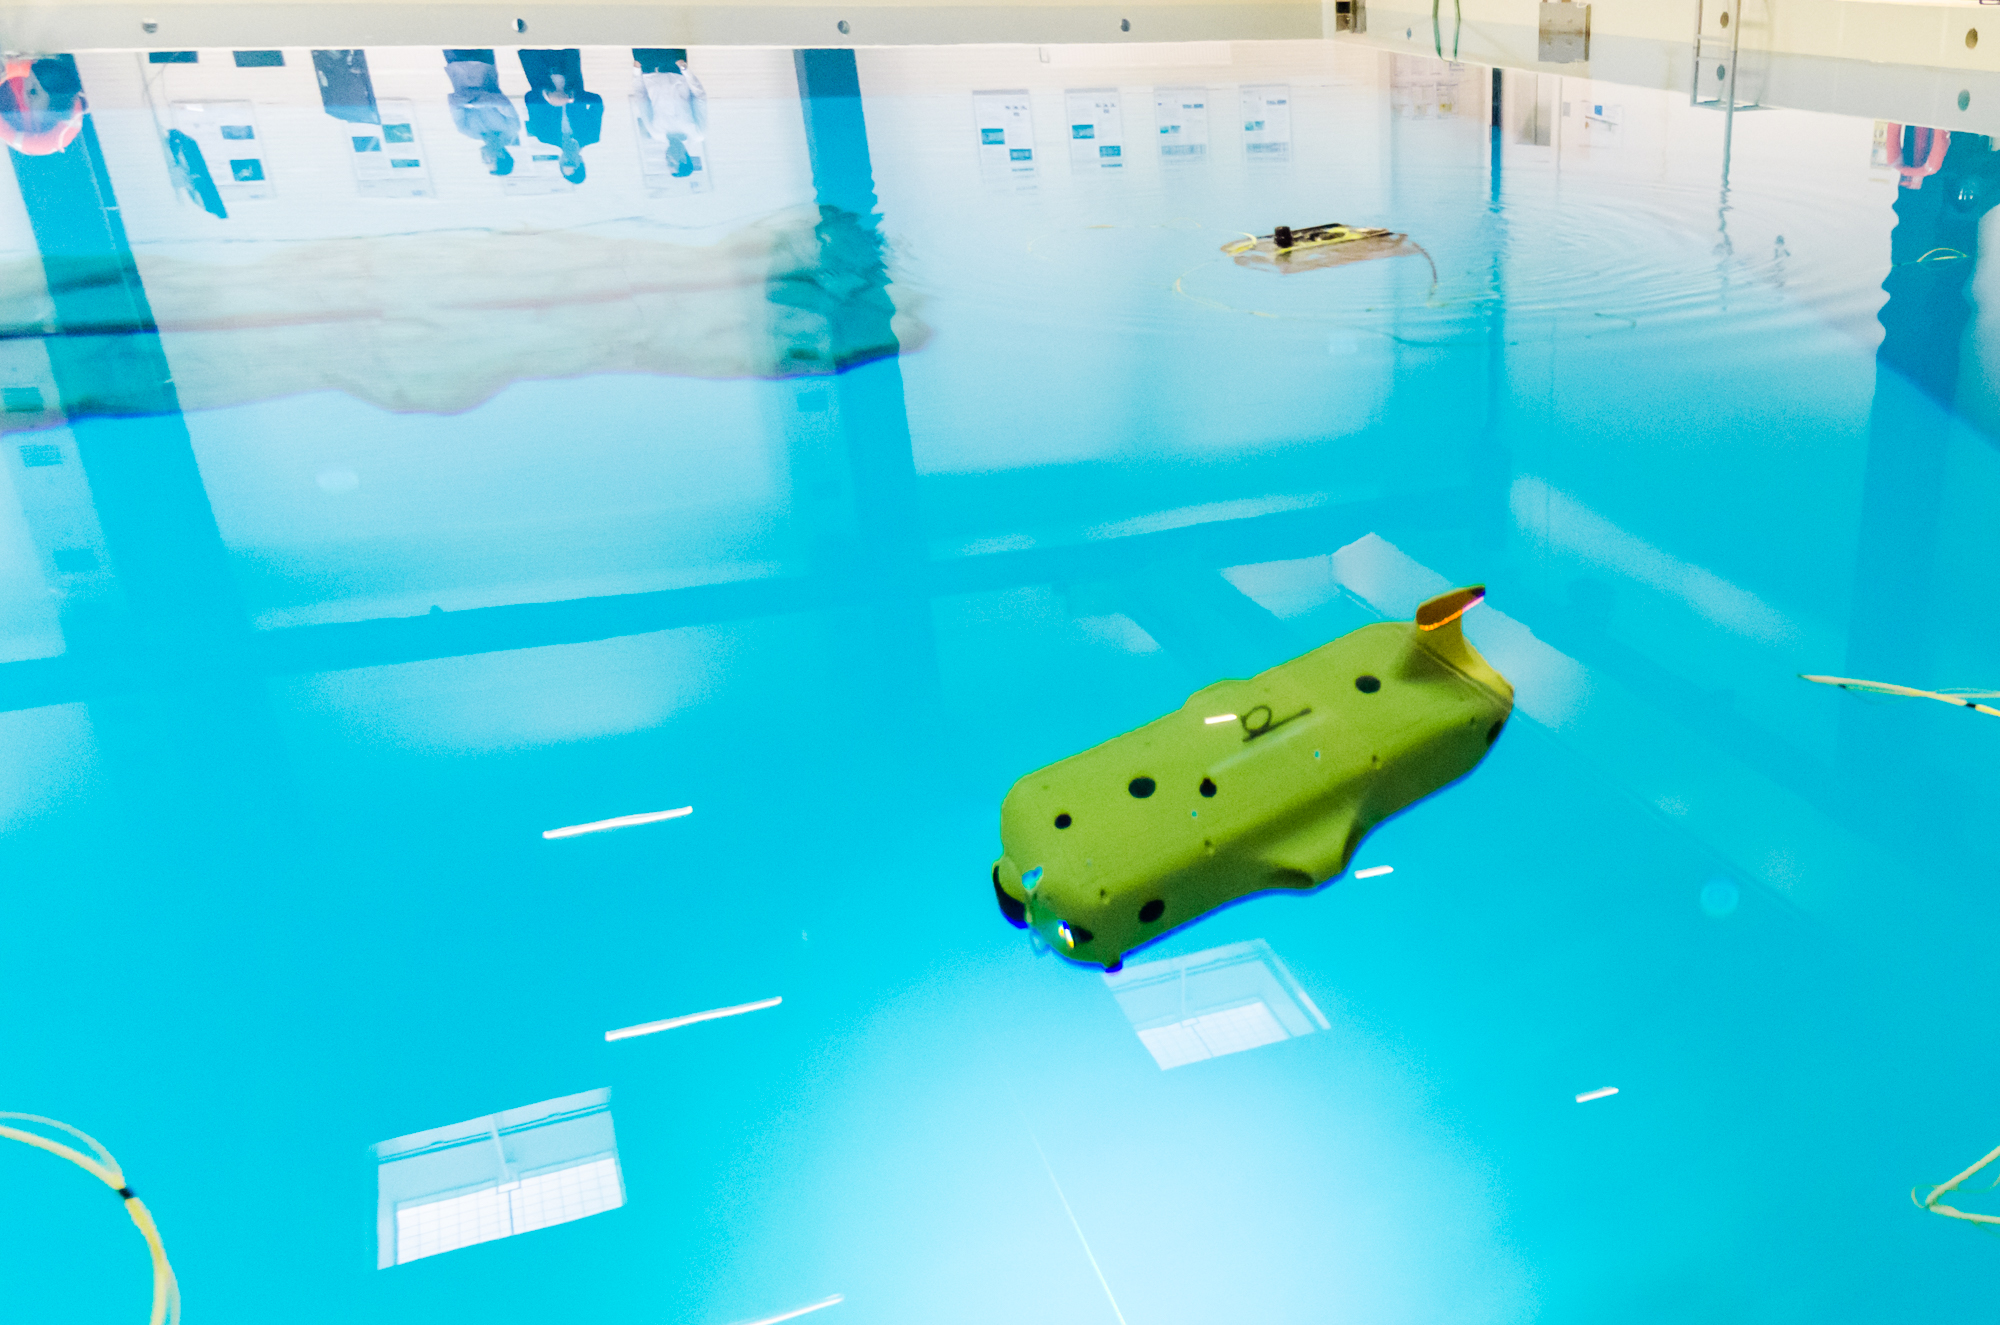
\includegraphics[width=0.9\columnwidth]{FlatFish-2.jpg}
	\caption{FlatFish in the maritime test tank at the DFKI facilities in Bremen during the 
	specification compliance tests. The pipeline mock-up is visible in the top left of the 
	picture.}
	\label{fig:flatfish2}
\end{figure}

% use section* for acknowledgement
\section*{Acknowledgment}

The FlatFish project is part of the ongoing research and development program of BG Group 
Brasil. It is funded by the Brazilian government via the Agência Nacional do Petróleo, Gás 
Natural e Biocombustíveis (ANP) and, due to its highly innovative nature, co-funded by the 
EMPRAPII (Empresa Brasileira de Pesquisa e Inovação Industrial) program.

The authors would like to thank BG Group for the excellent support of the project, with
special thanks to Gordon Laurenson, Phil Bremner, Diana Charles, Andrew Brown, Dawood 
Moataz, Steve Miller, Rosane Zagatti and John Costin.

% references section

\bibliographystyle{IEEEtran}
\bibliography{IEEEabrv,OCEANS2015_Washington_FlatrFish}



% that's all folks
\end{document}


